\subsection{Image Features}

An image feature is the combination of a keypoint and a feature descriptor \cite{loweObjectRecognitionLocal1999}. Keypoints are locations in an image which are intended to be invariant to lighting, scale, translation, and rotation\cite{shiGoodFeaturesTrack1994}, while descriptors are a data vector that acts as the unique fingerprint for the feature. Keypoints are located, and their descriptors generated in a process called feature extraction.

The output of feature extraction is a set of image features, which when combined are significantly smaller than the image from which they were extracted. Figure \ref{fig:feature_extraction_and_matching} shows the output of the ORB feature extractor, along with how the features extracted between two images can be matched by their descriptors. The capability to match the same set of points across multiple viewpoints is core to how 3D map points are estimated from multiple 2D images.

\begin{figure}[!ht]
    \centering
    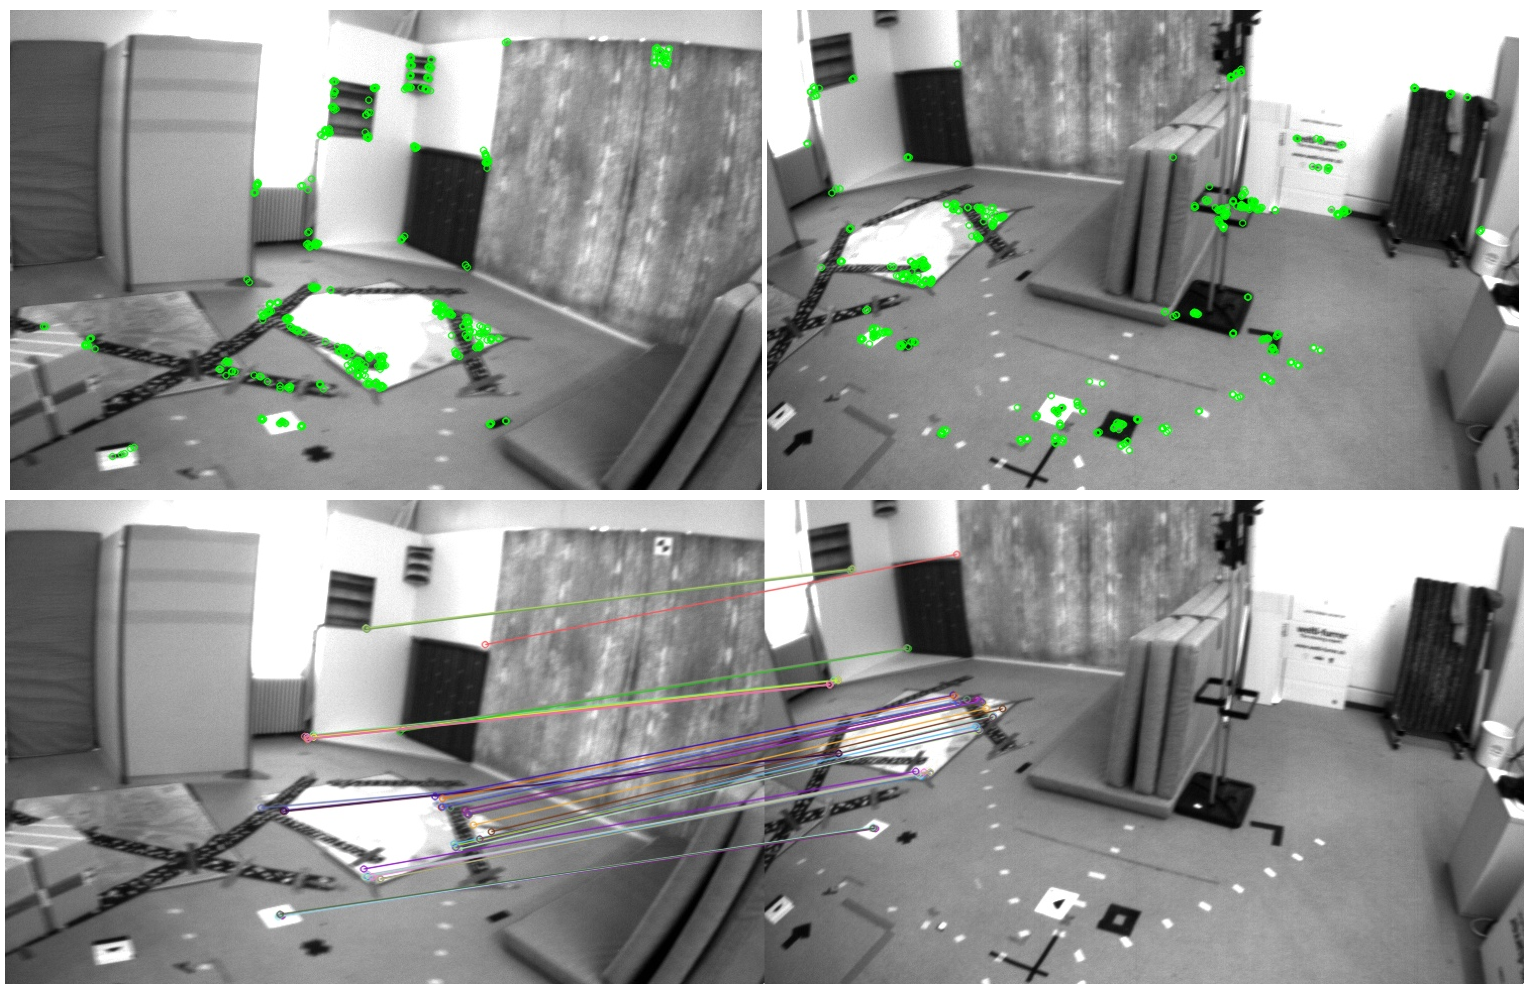
\includegraphics[width=0.9\textwidth]{resources/feature_extraction_and_matching.png}
    \caption[Image Feature Extraction and Matching]{(Top) ORB features extracted from two frames of the EuRoC MAV V1\_03 dataset \cite{burriEuRoCMicroAerial2016}. (Bottom) Corresponding ORB feature matches between the two frames.}
    \label{fig:feature_extraction_and_matching}
\end{figure}

It should be noted that map point matching is far from perfect. Feature descriptors tend to be based on the pixel values surrounding the keypoint location, meaning that visually similar image features will have similar descriptors. This is desirable and necessary to find feature matches between image frames, but means that in areas with repeating patterns or low visual texture, false matches are common.
